\documentclass{article}

\usepackage{graphicx}
\usepackage{tikz}
\usepackage{tikzsymbols}
\usetikzlibrary{calc,patterns,shapes.geometric}
\pagestyle{empty}
\usepackage[margin=0pt]{geometry}
\geometry{papersize={14in,12in}}

\def\centerarc[#1](#2)(#3:#4:#5){\draw[#1] ($(#2)+({#5*cos(#3)},{#5*sin(#3)})$) arc (#3:#4:#5);}

\begin{document}
	\begin{figure}
		\centering
		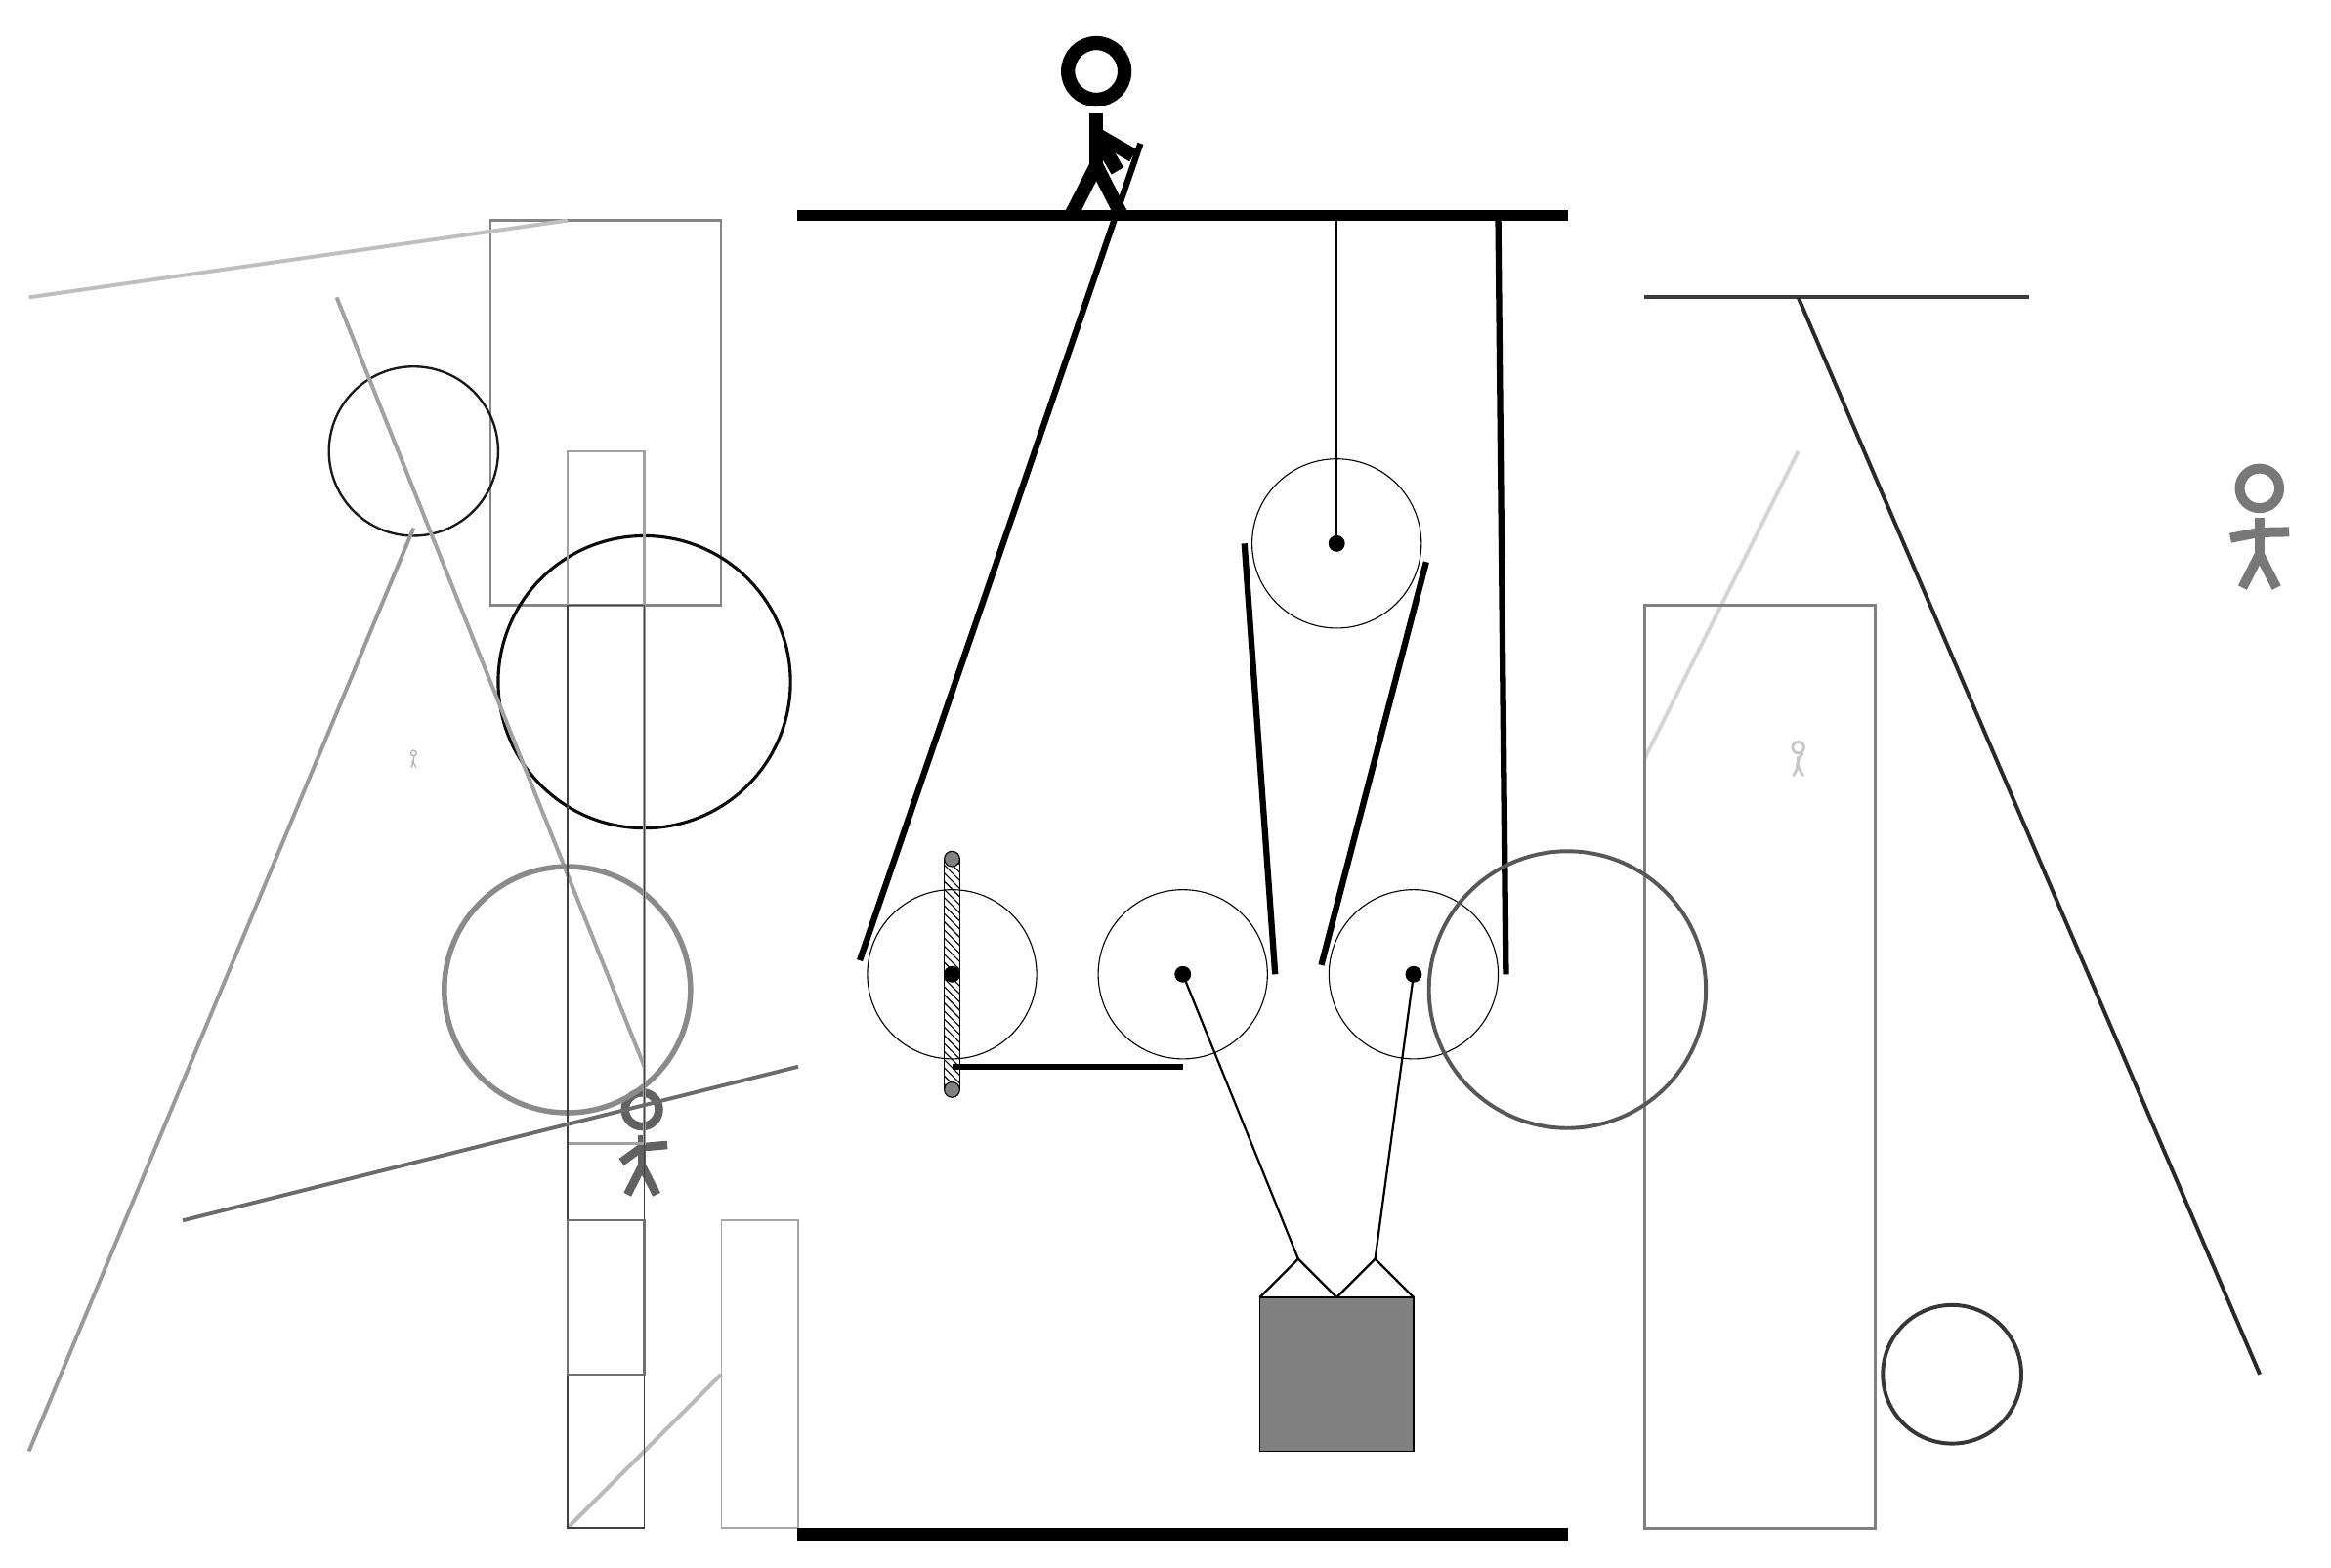
\begin{tikzpicture}
			%%%%% START %%%%%
			
			\draw[fill=black] (-4, 14) rectangle (6, 14.125);
			
			\draw (1, 4.2) circle (1.1);
			\draw[fill=black] (1, 4.2) circle (0.1);
			
			\draw (3, 9.8) circle (1.1);
			\draw[fill=black] (3, 9.8) circle (0.1);
			\draw[thick] (3, 9.8) -- (3, 14);
			
			\draw (4, 4.2) circle (1.1);
			\draw[fill=black] (4, 4.2) circle (0.1);
			
			\draw[thick] (4, 4.2) -- (3.5, 0.5);
			\draw[thick] (1, 4.2) -- (2.5, 0.5);
			\draw[thick]  (2, 0) -- (2.5, 0.5) -- (3, 0);
			\draw[thick]  (3, 0) -- (3.5, 0.5) -- (4, 0);
			\draw[fill=black!50] (2, 0) rectangle (4, -2);
			
			\draw (-2, 4.2) circle (1.1);
			\draw[fill=black] (-2, 4.2) circle (0.1);
			\draw[pattern=north west lines, pattern color=black] (-2.1, 5.7) rectangle (-1.9, 2.7);
			\draw[fill=black!50] (-2, 5.7) circle (0.1);
			\draw[fill=black!50] (-2, 2.7) circle (0.1);
			
			\draw[line width=0.8mm] (0.45, 15) -- (-3.2, 4.38);
			\centerarc[line width=0.8mm](-2, 4.2)(160:270:1.2000000000000002);
			\draw[line width=0.8mm](-2, 3.0) -- (1, 3.0);
			\centerarc[line width=0.8mm](1, 4.2)(270:360:1.2000000000000002);
			\draw[line width=0.8mm] (2.2, 4.2) -- (1.8, 9.8);
			\centerarc[line width=0.8mm](3, 9.8)(-20:180:1.2000000000000002);
			\draw[line width=0.8mm](4.164, 9.56) -- (2.8, 4.32);
			\centerarc[line width=0.8mm](4, 4.2)(160:360:1.2000000000000002);
			\draw[line width=0.8mm](5.2, 4.2) -- (5.1, 14);
			
			\draw[line width=0.5mm, color=black!77](7, 13) -- (12, 13);
			
			\node[line width=0.4mm, color=black!29] at (-9, 7) {\Strichmaxerl[1][68][83]};
			\draw[line width=0.3mm, color=black!48] (-5, 9) rectangle (-8, 14);
			\draw[line width=0.5mm, color=black!27](-7, -3) -- (-5, -1);
			\draw[line width=0.5mm, color=black!25](-7, 14) -- (-14, 13);
			\draw [line width=0.4mm, color=black!96](-6, 8) circle (1.9);
			\draw[line width=0.5mm, color=black!17](7, 7) -- (9, 11);
			
			\draw [line width=0.5mm, color=black!79](11, -1) circle (0.9);
			\node[line width=0.3mm, color=black!22] at (9, 7) {\Strichmaxerl[2][79][57]};
			\draw[line width=0.5mm, color=black!84](9, 13) -- (15, -1);
			
			\draw [line width=0.3mm, color=black!90](-9, 11) circle (1.1);
			
			\draw[line width=0.5mm, color=black!37](-6, 3) -- (-10, 13);
			\node[line width=0.7mm, color=black!62] at (-6, 2) {\Strichmaxerl[6][36][5]};
			
			\draw[line width=0.5mm, color=black!40](-9, 10) -- (-14, -2);
			\draw [line width=0.7mm, color=black!46](-7, 4) circle (1.6);
			\draw[line width=0.3mm, color=black!37] (-6, 11) rectangle (-7, 2);
			
			\draw[line width=0.2mm, color=black!75] (-6, -3) rectangle (-7, 9);
			
			\draw[line width=0.5mm, color=black!58](-4, 3) -- (-12, 1);
			\node[line width=0.2mm, color=black!53] at (15, 10) {\Strichmaxerl[7][11][1]};
			
			\draw[line width=0.4mm, color=black!50] (7, 9) rectangle (10, -3);
			\draw[line width=0.3mm, color=black!56] (-6, -1) rectangle (-7, 1);
			
			\draw [line width=0.5mm, color=black!66](6, 4) circle (1.8);
			
			\draw[line width=0.2mm, color=black!35] (-5, -3) rectangle (-4, 1);
			
			\node at (-0.07, 15.2) {\Strichmaxerl[10][120][-30]};
			
			\draw[fill=black] (-4, -3) rectangle (6, -3.15);
			
			%%%%% END %%%%%
		\end{tikzpicture}
	\end{figure}	
\end{document}